\documentclass[smaller,dvipsnames,ratio=169]{beamer}

\usetheme[numbering=fraction,%
          block=fill,%
          sectionpage=progressbar,%
          subsectionpage=progressbar,%
  ]{metropolis} % Use metropolis theme
\setbeamercovered{invisible}

\usepackage[utf8]{inputenc}
\usepackage{xcolor}
\usepackage{xspace}
\usepackage{booktabs}
\usepackage{amssymb}
\usepackage{listings}
\usepackage{todonotes}

\usepackage{tikz,comment}
\usetikzlibrary{shapes.multipart,shapes.geometric,positioning,backgrounds,fit,calc,arrows.meta}



\newcommand{\htw}{\emph{Hunt the Wumpus }}

\title{Hakuna Matata: A Logic-Based Agent for the \htw Game}
\subtitle{Team White}
\author{Filippo~De~Bortoli \and Aneta~Koleva \and Lorenz~Leutgeb}
\institute{Free University of Bozen-Bolzano\\[2mm] \texttt{\{\href{mailto:filippo.debortoli@stud-inf.unibz.it}{filippo.debortoli},\href{mailto:aneta.koleva@stud-inf.unibz.it}{aneta.koleva},\href{mailto:lorenz.leutgeb@stud-inf.unibz.it}{lorenz.leutgeb}\}\newline @stud-inf.unibz.it}}
\date{01.06.2018}

\begin{document}

  \maketitle

  \begin{frame}{Outline}
    \tableofcontents
  \end{frame}

  \section{Introduction}

  \begin{frame}{Task}
    \begin{enumerate}
      \item Develop an intelligent agent that plays the game \htw.
      \item Implement a strategy to complete the knowledge about the state of the world and to be able to reason with respect to it. 
      \item Find an optimal strategy, i.e.\ maximize score.
    \end{enumerate}
  \end{frame}
%not sure if a slide with explanation of the game is needed

  \begin{frame}{Tools of the Trade}
  \begin{enumerate}
    %\item Pragmatic choices to avoid any confusions
    %\item Keeping it DRY (Don't Repeat Yourself)
    %\item Avoid reinvention
    \item Simulator rewritten in Python 3.6 (removes C dependency)
  \end{enumerate}

  \begin{center}
  \begin{tabular}{lll}
    \textbf{Tool/Library} & \textbf{Version} & \textbf{Purpose} \\
    Python & 3.6 & Runtime \\
    DLV & Dec 2012 & ASP solver \\
    NetworkX & 2.1 & Graph algorithms \\
  \end{tabular}
  \end{center}
  \end{frame}

  \section{Ideas and used concepts}
	 \begin{frame}{World Knowledge}
	
	  \begin{itemize}
		\item Static, partly-observable environment.
		\item Incomplete initial knowledge.
		\item Safety first!
		\item The agent discovers size of the world when it bumps. 
		\item Unsafe rooms and how to reason to avoid them. 
	  \end{itemize}
	 \end{frame}

 \begin{frame}{Why ASP and DLV?}
	\begin{itemize}
		\item Previous experience with ASP.
		\item Allows to model non-monotonic reasoning through CWA. 
		\item Combines a high-level
		logic with grounding and solving. 
		\item ASP allows processing of incomplete knowledge. 
		\item At each time step, DLV called after perception has been caught.
		
	\end{itemize}
 \end{frame}

  \begin{frame}{$A^{\star}$ Search and World Exploration}
	 \begin{itemize}
	 	\item Build a reachability graph such that:
		 	\begin{itemize}
				 \item Vertices are all the safe and reachable rooms that still haven't been explored.
				 \item Edges are the connections between these rooms.
		    \end{itemize}
	    \item Calculate the weights using the cost function: 
	    $$
	    	g(C,C^\prime) := M((X,Y),(X^\prime,Y^\prime)) + R((X,Y),O,(X^\prime,Y^\prime))
	    $$
	    \item Compute the minimal cost of reaching the target room using \emph{$A^{\star}$ search} : 
	    \(f(n) = g(n) + h(n)\)
	    \item Deciding a goal room depending on the current mode of the agent.
	    \item Choosing next room depending on the goal.
		 
	 \end{itemize}
  \end{frame}

\begin{frame}{Cost graph example}
	\begin{figure}\centering
		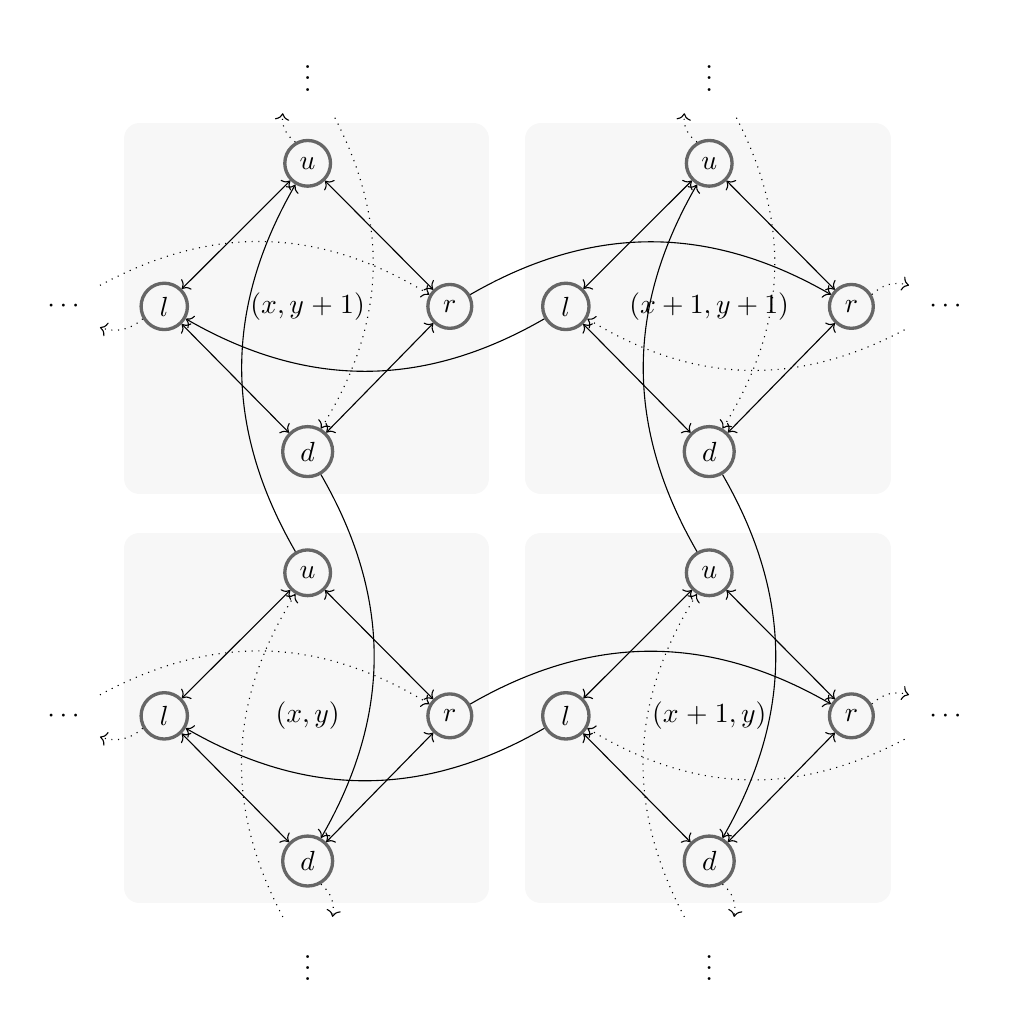
\begin{tikzpicture}[roundnode/.style={circle, draw=black!60, very thick,minimum size=4mm}]
	\begin{scope}
		\node[regular polygon, regular polygon sides=4, align=center, text width={width("$(x + 1, y + 1)$")}] (n11) {$(x, y)$};
		\node[roundnode] (u11) [above=-1mm of n11] {$u$};
		\node[roundnode] (l11) [left=-1mm of n11] {$l$};
		\node[roundnode] (r11) [right=-1mm of n11] {$r$};
		\node[roundnode] (d11) [below=-1mm of n11] {$d$};
		\draw [<->] (u11) -> (l11);
		\draw [<->] (u11) -> (r11);
		\draw [<->] (d11) -> (l11);
		\draw [<->] (d11) -> (r11);
	\end{scope}
		
	\begin{scope}[xshift=5.1cm]
		\node[regular polygon, regular polygon sides=4, align=center, text width={width("$(x + 1, y + 1)$")}] (n21) {$(x + 1, y)$};
		\node[roundnode] (u21) [above=-1mm of n21] {$u$};
		\node[roundnode] (l21) [left=-1mm of n21] {$l$};
		\node[roundnode] (r21) [right=-1mm of n21] {$r$};
		\node[roundnode] (d21) [below=-1mm of n21] {$d$};
		\draw [<->] (u21) -> (l21);
		\draw [<->] (u21) -> (r21);
		\draw [<->] (d21) -> (l21);
		\draw [<->] (d21) -> (r21);
	\end{scope}
		
	\begin{scope}[yshift=5.2cm]
		\node[regular polygon, regular polygon sides=4, align=center, text width={width("$(x + 1, y + 1)$")}] (n12) {$(x, y + 1)$};
		\node[roundnode] (u12) [above=-1mm of n12] {$u$};
		\node[roundnode] (l12) [left=-1mm of n12] {$l$};
		\node[roundnode] (r12) [right=-1mm of n12] {$r$};
		\node[roundnode] (d12) [below=-1mm of n12] {$d$};
		\draw [<->] (u12) -> (l12);
		\draw [<->] (u12) -> (r12);
		\draw [<->] (d12) -> (l12);
		\draw [<->] (d12) -> (r12);
	\end{scope}
		
	\begin{scope}[yshift=5.2cm,xshift=5.1cm]
		\node[regular polygon, regular polygon sides=4, align=center] (n22) {$(x + 1, y + 1)$};
		\node[roundnode] (u22) [above=-1mm of n22] {$u$};
		\node[roundnode] (l22) [left=-1mm of n22] {$l$};
		\node[roundnode] (r22) [right=-1mm of n22] {$r$};
		\node[roundnode] (d22) [below=-1mm of n22] {$d$};
		\draw [<->] (u22) -> (l22);
		\draw [<->] (u22) -> (r22);
		\draw [<->] (d22) -> (l22);
		\draw [<->] (d22) -> (r22);
	\end{scope}
		
	\begin{scope}[xshift=8.1cm]
		\node[regular polygon, regular polygon sides=4] (n31) {$\cdots$};
	\end{scope}
		
	\begin{scope}[yshift=5.2cm,xshift=8.1cm]
		\node[regular polygon, regular polygon sides=4] (n32) {$\cdots$};
	\end{scope}

	\begin{scope}[yshift=8.2cm]
		\node[regular polygon, regular polygon sides=4] (n13) {$\vdots$};
	\end{scope}

	\begin{scope}[yshift=8.2cm,xshift=5.1cm]
		\node[regular polygon, regular polygon sides=4] (n23) {$\vdots$};
	\end{scope}

	\begin{scope}[xshift=-3.1cm]
		\node[regular polygon, regular polygon sides=4] (n01) {$\cdots$};
	\end{scope}

	\begin{scope}[yshift=-3.1cm,xshift=5.1cm]
		\node[regular polygon, regular polygon sides=4] (n20) {$\vdots$};
	\end{scope}

	\begin{scope}[yshift=-3.1cm]
		\node[regular polygon, regular polygon sides=4] (n10) {$\vdots$};
	\end{scope}

	\begin{scope}[yshift=5.2cm,xshift=-3.1cm]
		\node[regular polygon, regular polygon sides=4] (n02) {$\cdots$};
	\end{scope}

	\path [->] (r11) edge [bend left] (r21);
	\path [->] (l21) edge [bend left] (l11);
	\path [->] (u11) edge [bend left] (u12);
	\path [->] (d12) edge [bend left] (d11);
	\path [->] (u21) edge [bend left] (u22);
	\path [->] (d22) edge [bend left] (d21);
	\path [->] (r12) edge [bend left] (r22);
	\path [->] (l22) edge [bend left] (l12);

	\path [->, dotted] (r21) edge [bend left] (n31);
	\path [->, dotted] (r22) edge [bend left] (n32);
	\path [->, dotted] (u12) edge [bend left] (n13);
	\path [->, dotted] (u22) edge [bend left] (n23);
	\path [->, dotted] (l11) edge [bend left] (n01);
	\path [->, dotted] (d11) edge [bend left] (n10);
	\path [->, dotted] (l12) edge [bend left] (n02);
	\path [->, dotted] (d21) edge [bend left] (n20);

	\path [<-, dotted] (l21) edge [bend right] (n31);
	\path [<-, dotted] (l22) edge [bend right] (n32);
	\path [<-, dotted] (d12) edge [bend right] (n13);
	\path [<-, dotted] (d22) edge [bend right] (n23);
	\path [<-, dotted] (r11) edge [bend right] (n01);
	\path [<-, dotted] (u11) edge [bend right] (n10);
	\path [<-, dotted] (r12) edge [bend right] (n02);
	\path [<-, dotted] (u21) edge [bend right] (n20);

	\begin{pgfonlayer}{background}
		\filldraw[line width=4mm,join=round,black!3]
			(u11.north -| r11.east) rectangle (d11.south -| l11.west)
			(u21.north -| r21.east) rectangle (d21.south -| l21.west)
			(u12.north -| r12.east) rectangle (d12.south -| l12.west)
			(u22.north -| r22.east) rectangle (d22.south -| l22.west)
		;
	\end{pgfonlayer}
\end{tikzpicture}

		\caption{Visualization of cost}
	\end{figure}
\end{frame}


  \begin{frame}{Different modes}
   \begin{enumerate}
   	\item Explore - until the gold is discovered or there are more unexplored rooms 
   	\item Grab - when glitter is perceived
   	\item Kill - not in any other mode and the gold is still up for grabs
		   	\begin{itemize}
		   		\item can try to kill the wumpus?
		   		\item should it try to kill the wumpus?
		   		\item can it shoot?
		   	\end{itemize}
   	\item Escape - not in any other mode.
   \end{enumerate}
  \end{frame}

\iffalse
  \begin{frame}{ASP Encoding}
    \begin{center}
      \begin{tabular}{ll}
        \textbf{Predicate} & \textbf{Meaning} \\
        now/3 & position and orientation of the agent \\
        stench/2 & stench has been found in here \\
        wumpusDead/0 & a scream has been perceived \\
        grabbed/0 & glitter perceived, gold has been grabbed \\
      \end{tabular}
    \end{center}
  \end{frame}

  \begin{frame}{Heuristics}
    % TODO.
  \end{frame}
\fi
  \section{Implementation}
	%something more here maybe? it's a section with one slide (diagram)
  \begin{frame}{Architecture of the implementation}
  	\begin{figure}\centering
  		
		
			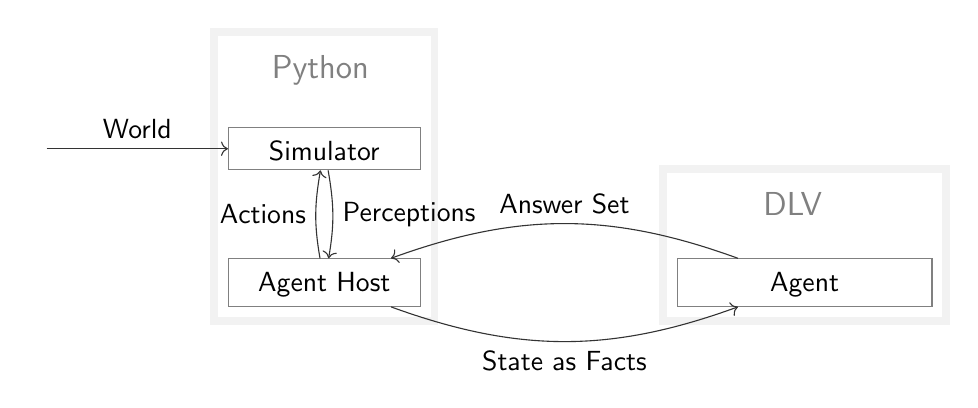
\begin{tikzpicture}[
			node distance=1cm and 5mm,
			every node/.style={font=\sffamily},
			title/.style={font=\color{black!50}\sffamily},
			typetag/.style={rectangle, draw=black!50, font=\sffamily, anchor=west, text height=3mm, align=center}
			]
			
			\node (lp) at (0, -1cm) {};
			\node (as) at (0, -3.2cm) {};
			
			\node (gl) at (3.6cm, 0) [align=center, text width=2.1cm, title] { \large Python };
			
			\node (par) [below=of gl.west, text width=22mm, typetag] { Simulator };
			\node (gro) [below=1.7cm of par.west, text width=22mm, typetag] { Agent Host };
			
			\node (g) [draw=gray!10, line width=1mm, inner sep=5pt, fit={(gl) (par) (gro)}] {};
			
			\node (sl) at (9.6cm, -1.7cm) [align=center, text width=2.7cm, title] { \large DLV };
			
			\node (ngs) [below=of sl.west, text width=3cm, typetag] { Agent };
			
			\node (s) [draw=gray!10, line width=1mm, inner sep=5pt, fit={(sl) (ngs)}] {};
			
			\draw [->, draw=black!80] (gro) to [out=340, in=200] node [midway, below] {State as Facts} (ngs);
			\draw [->, draw=black!80] (ngs) to [out=160, in=20] node [midway, above] {Answer Set} (gro);
			
			\draw [->, draw=black!80] (par) to [out=280, in=80] node [midway, right] {Perceptions} (gro);
			\draw [<-, draw=black!80] (par) to [out=260, in=100] node [midway, left] {Actions} (gro);
			
			\draw [->, draw=black!80] (lp) -- (par) node [midway, above] {World};
			\end{tikzpicture}
	
  		\caption{Architecture }
  	\end{figure}	
  \end{frame}

  \begin{frame}{Autopilot}
  	\begin{itemize}
  		\item Careful selected rules for the goal and detection of unsafe rooms.
  		\item Prevent planning of paths that pass thorough unsafe rooms.		  		
		\item Decreases the overall run time of the agent.

  	\end{itemize}
  	
  \end{frame}


  \section{Evaluation}
  
  \begin{frame}{Perfect agent}
    
    \begin{itemize}
      \item Omniscience, i.e. complete knowledge of the world. 
      \item Optimal solution as shortest path over the action graph:
      \begin{itemize}
      	\item Nodes - room with orientation (X,Y,O)
      	\item Edges - connections between neighboring rooms
      	\item Weight = 1 - if the target is not in the same room where the Wumpus is 
      	\item Weight = 10 - otherwise
      \end{itemize}
	  \item If the gold is unreachable, climbs out immediately.
      \item Score of this agent taken as reference for a dungeon.
    \end{itemize}
  \end{frame}


  \begin{frame}{The test suite and results}
    \begin{table}[t]
      	\label{tbl:test}
      	\centering
      	\begin{tabular}{rrrrr}
      		\toprule
      		\multicolumn{1}{c}{World size} & \multicolumn{1}{c}{instances} & \multicolumn{1}{c}{avg. gap} & \multicolumn{1}{c}{stddev gap} & \multicolumn{1}{c}{avg. wall-time (s)}\\
      		\midrule
      		4 & 160	& 419 & 488 & 0.1440 \\
      		5 & 80  & 464 & 493 & 0.2656 \\
      		6 & 80  & 634 & 474 & 0.4600 \\
      		7 & 40  & 630 & 468 & 2.8005 \\
      		8 & 40  & 653 & 471 & 3.8736 \\
      		9 & 20  & 557 & 490 & 4.7723 \\
      		10 & 20 & 714 & 452 & 11.3828 \\
      		11 & 10 & 785 & 414 & 0.1573 \\
      		12 & 10 & 595 & 498 & 0.5594 \\
      		13 & 5  & 383 & 524 & 0.0158 \\
      		14 & 5  & 600 & 506 & 11.8238 \\
      		\bottomrule\\
      	\end{tabular}
      	\caption{Some aggregated results obtained by assessing Hakuna against our testing suite.}
      \end{table}
   \end{frame}

	\begin{frame}{Performance assessment}
		\begin{itemize}
			\item Performance of the agent compared against the perfect agent.
			\item Reasons for Hakuna's under-performing: 
			\begin{itemize}
				\item Possible pits blocking its way to the gold.
				\item Checks all possible rooms before giving up when the gold is unreachable.
			
			\end{itemize}
		\end{itemize}
	\end{frame}

	

  \section{Conclusion}

  \begin{frame}{Possible Improvements}
      % TODO: I think this can be skipped, if we do a good job.
  \end{frame}

  \begin{frame}{Conclusion}
  \end{frame}

  \begin{frame}[standout]
    Thank you!
  \end{frame}

\end{document}
